\section{Density and Double occupency}
\begin{figure}[H]
%\centering
\begin{subfigure}{.5\textwidth}
 % \centering
 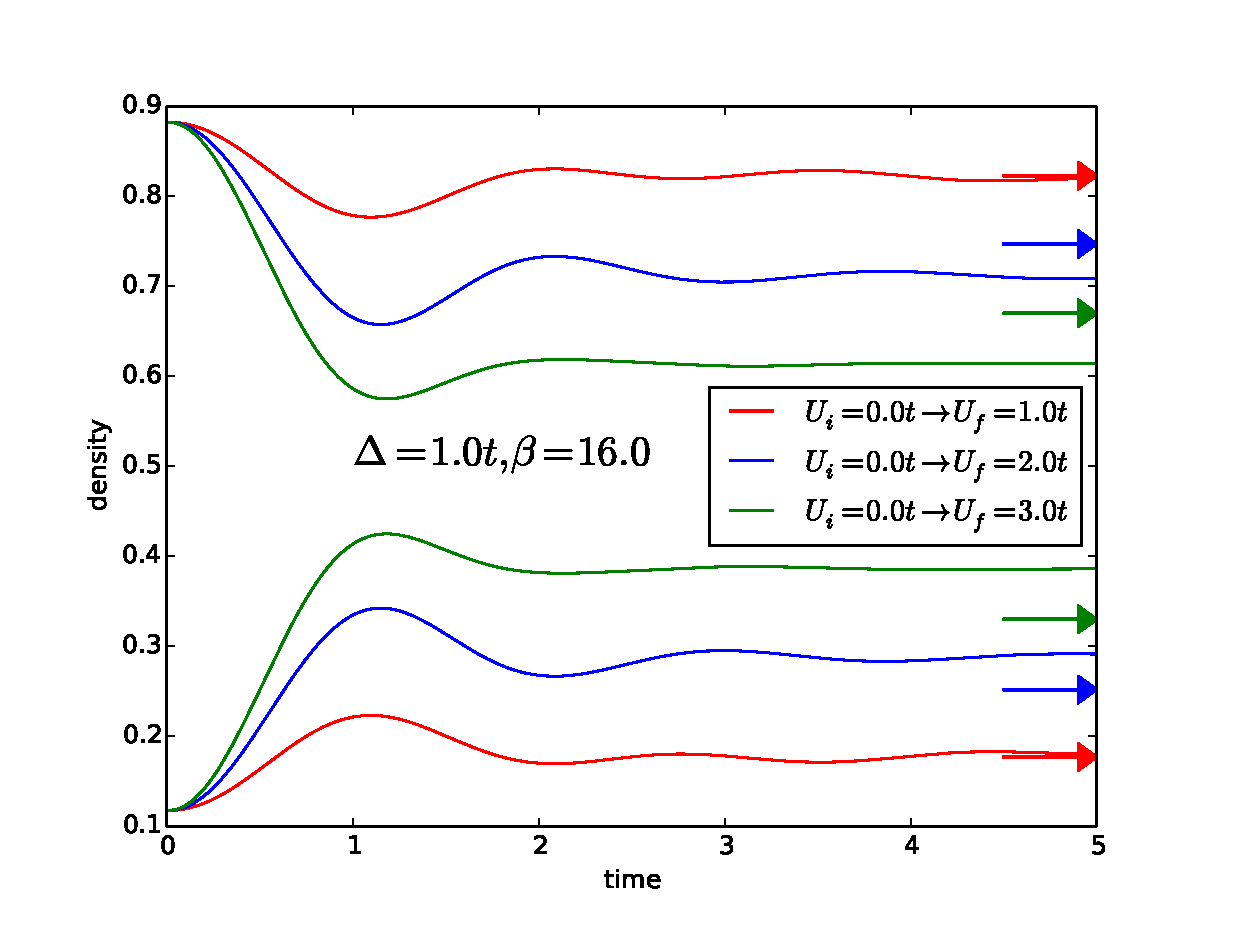
\includegraphics[width=1.1\linewidth]{interaction_quench/density_interaction.eps}
  \caption{density of A and B sublattice as function of time for different sudden interaction quench $U_i \rightarrow U_f$. All the cases initial state at $\beta=16$ with $\Delta=1.0$ }
  %\label{fig:sub1}
\end{subfigure}%
\begin{subfigure}{.5\textwidth}
 % \centering
  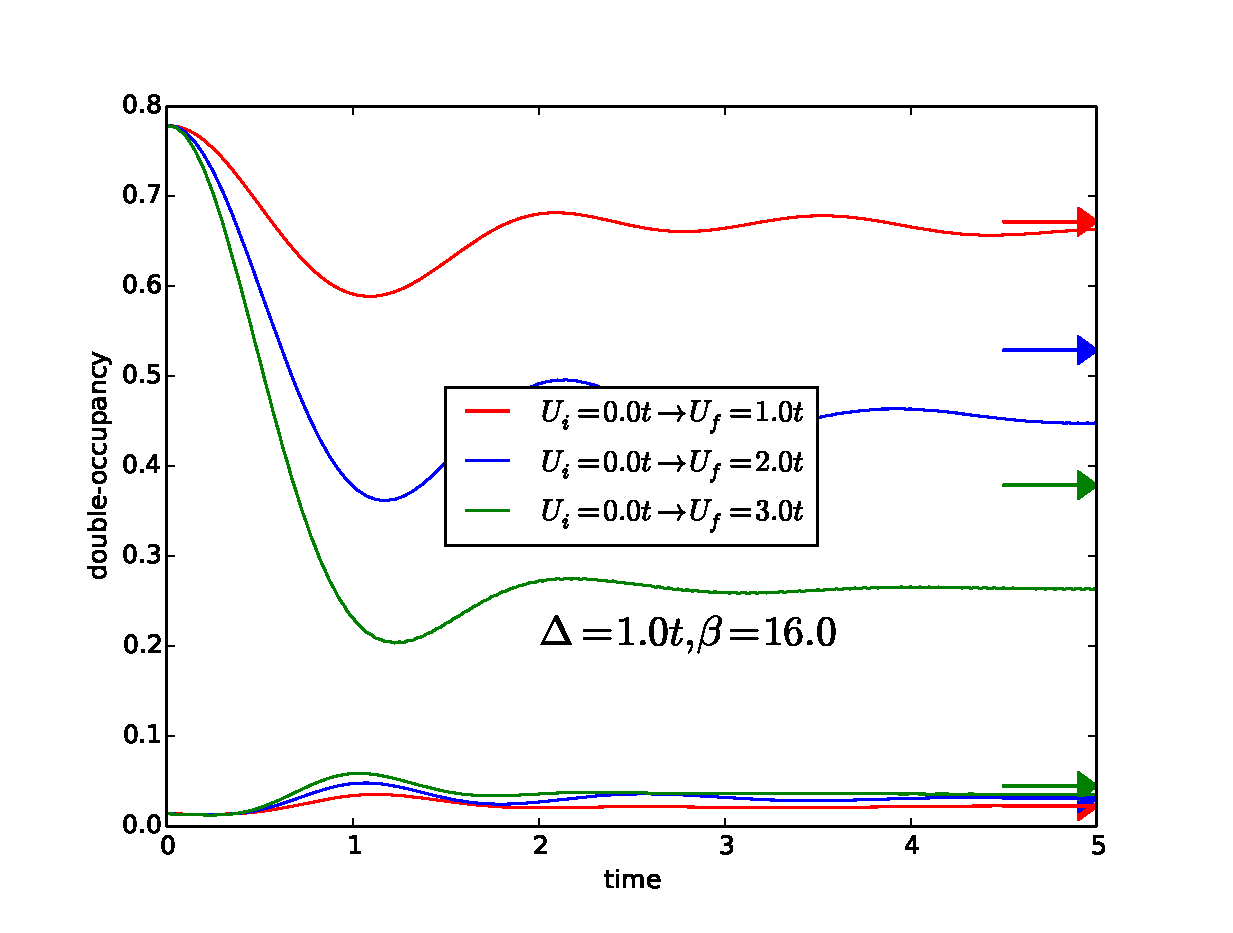
\includegraphics[width=1.1\linewidth]{interaction_quench/double-occupancy_interaction.eps}
  \caption{Double occupancy at A and B sublattice as function of time. }
  %\label{fig:sub2}
\end{subfigure}
\caption{}
\label{density}
\end{figure}



In fig \ref{density} density at A and B sub-lattice evolution is plotted as as interaction is quenched from $U_i$ = 0 to $U_f$ = 1.0, 2.0,3.0 where ionic staggered potential is kept fixed at $\Delta=1.0t$. All the cases intial state is at beta=16. IN the density plot lower set of lines are for A sub lattice and uper set are for B sublattice which is negetive orbita potetial compare to A. Corresponding arrows are for euilibium density at A and B sublattice at beta=16. Effective temperature of the system after interaction quench is calculated below and at those temperature equllibium density is give.
%for the Hubbard model we see that steady double occupancy is larger than the equilibrium value. where as for IHM case its is lower 

\section{Energy}
Energy at $\gamma$ =\{ A, B\}  sublattice is defined as
\be 
E_{\gamma} = \Delta * n_{\gamma} + E_{k\gamma} + U_f*d_{\gamma}\\
\en 
where $n_{\gamma}$ is the occupation andd $d_{\gamma}$ is double occupation at $\gamma$ sublattice and $E_{k\gamma}$ is kinetic energy = $-2\int G_{\gamma}(\tau) G_{\bar{\gamma}}(\beta - \tau)$

\begin{figure}[H]
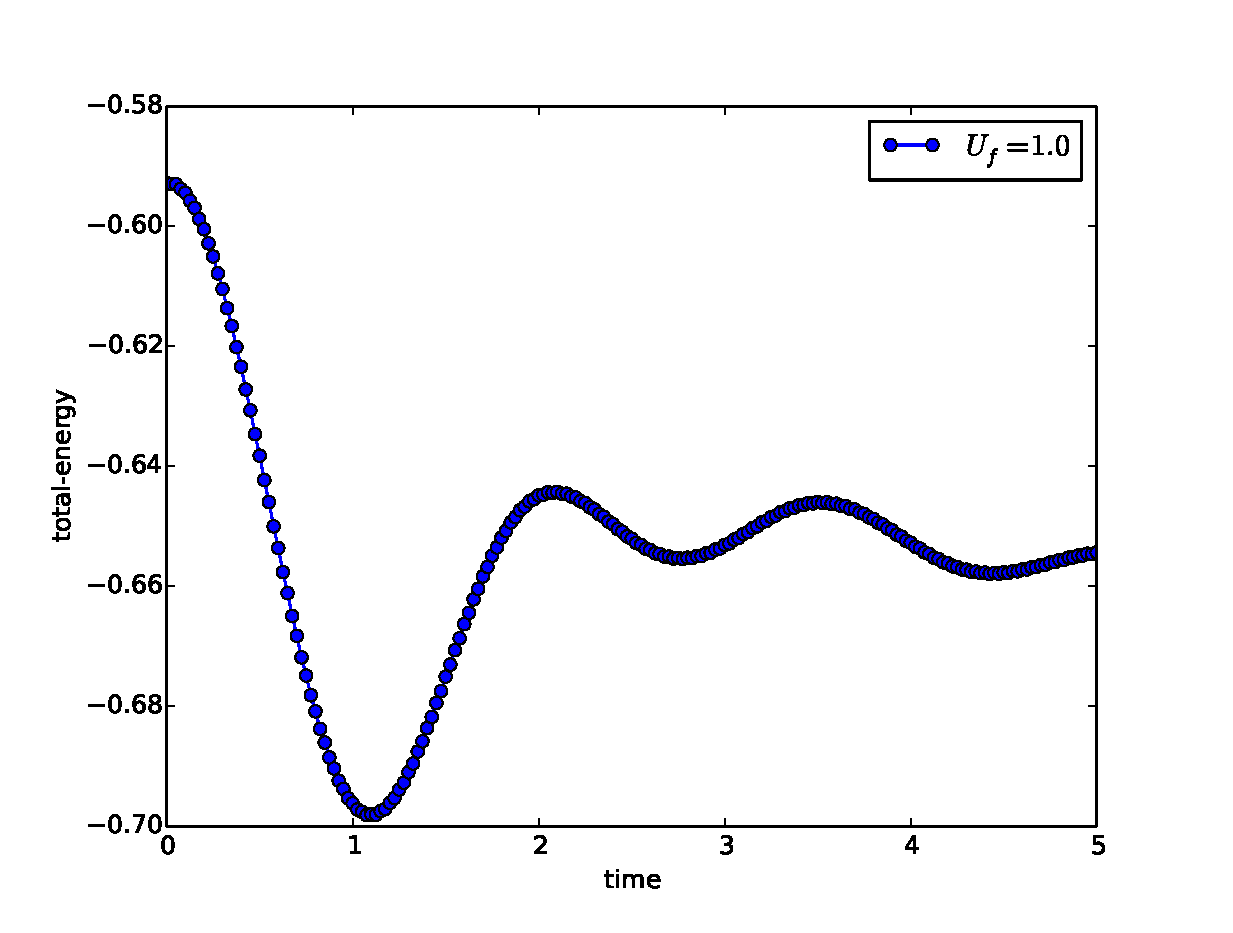
\includegraphics[width=0.8\linewidth]{interaction_quench/total-energy_new1.eps}
  \caption{here total energy = ($E_A + E_B$)/2.0}
\end{figure}


